\subsection{Sviluppo} \label{sviluppo}

	\subsubsection{Scopo del processo}

		Il seguente processo contiene le attività di analisi dei requisiti, progettazione e codifica. Queste,
		partendo da quanto descritto nel Capitolato e tramite la conduzione del processo di Gestione,
		risulteranno nello sviluppo del prodotto software.

    \subsubsection{Analisi dei requisiti}

        In seguito al completamento dello \StudioFattibilita{}, è compito degli Analisti redigere il documento di
        \AnalisiRequisiti . Esso ha l'intento di formalizzare e rendere tracciabili i requisiti e i casi d'uso individuati,
        presentandoli seguendo le specifiche sottostanti.
			
        \myparagraph{Requisiti}

            Ogni requisito è classificato tramite il seguente formalismo:

                \begin{center}
                    \textbf{R$\{$X$\}$$\{$Y$\}$$\{$codice\_identificativo$\}$}
                \end{center}

            dove:

                \begin{itemize}
                    \item \textbf{X} specifica la tipologia di requisito:
                        \begin{itemize}
                            \item \textit{F}: requisito funzionale;
                            \item \textit{P}: requisito prestazionale;
                            \item \textit{Q}: requisito qualitativo;
                            \item \textit{V}: vincolo progettuale.
                        \end{itemize}
                    \item \textbf{Y} indica uno dei seguenti gradi di necessità:
                        \begin{itemize}
                            \item \textit{O}: requisito obbligatorio;
                            \item \textit{D}: requisito desiderabile;
                            \item \textit{F}: requisito facoltativo.
                        \end{itemize}
                    \item \textbf{codice\_identificativo}: è un codice composto da una serie di numeri separati tramite
                    punto che identificano il requisito in maniera univoca e lo esprimono gerarchicamente.
                \end{itemize}
				
            È imperativo che un requisito non possa cambiare denominazione col passare del tempo.
            La lista dei requisiti è espressa in forma tabellare e ciascun requisito è esplicato nel seguente modo:

                \begin{itemize}
                    \item \textbf{ID Requisito}: rappresenta un identificativo del requisito, costruito come sopra;
                    \item \textbf{Descrizione}: breve ma chiara e precisa; non deve lasciare spazio ad ambiguità;
                    \item \textbf{Fonte}: indica la fonte da cui è stato estrapolato il requisito e può essere:
                        \begin{itemize}
                            \item \textbf{capitolato}: derivante direttamente dal capitolato;
                            \item \textbf{verbale}: derivante da un incontro verbalizzato;
                            \item \textbf{caso d'uso}: derivante da uno o più casi d'uso.
                        \end{itemize}
                \end{itemize}

            \textbf{Esempi di requisiti:}

                \begin{center}
                    \rowcolors{2}{gray!25}{gray!5}
                        \begin{tabular}{ >{\centering\arraybackslash}m{3cm} m{7cm} m{3cm} >{\centering\arraybackslash}m{2.5cm} }
                            \rowcolor{gray!50}
                            ID Requisito & Descrizione & Fonti \\
                            RVO1.2 & Esempio 1 & Capitolato; UC1 \\
                            RPF3.1 & Esempio 2 & Capitolato; UC2 \\
                        \end{tabular}
                \end{center}
				
        \myparagraph{Casi d'uso}

            Ogni caso d'uso è classificato tramite il seguente formalismo:

                \begin{center}
                    \textbf{UC$\{$codice\_identificativo$\}$}
                \end{center}

            dove:

                \begin{itemize}
                    \item \textbf{codice\_identificativo} è un codice composto da una serie di numeri separati tramite
                    punto che identificano il caso d'uso in maniera univoca e lo esprimono gerarchicamente.
                \end{itemize}

            È imperativo che un caso d'uso non possa cambiare denominazione col passare del tempo.
            Per i casi d'uso che si sviluppano in sotto-casi viene incluso un diagrammma UML
            denominato \glossaryItem{Use Case Diagram}.
            Ciascun caso d'uso è esplicato dai seguenti punti:

                \begin{itemize}
                    \item\textbf{ID Caso d'uso}: identificativo del caso d'uso, costruito come scritto sopra;
                    \item\textbf{Titolo}: titolo del caso d'uso;
                    \item\textbf{Descrizione}: breve descrizione del caso d'uso;
                    \item\textbf{Attori}: lista di \glossaryItem{attori} principali e secondari coinvolti nel caso d'uso;
                    \item\textbf{Precondizione}: condizione che deve essere verificata prima dell'esecuzione del caso d'uso;
                    \item\textbf{Postcondizione}: condizione che deve essere verificata dopo dell'esecuzione del caso d'uso;
                    \item\textbf{Scenario principale}: descrizione composta dal flusso dei casi d'uso figli;
                    \item\textbf{Scenari alternativi}: descrizione composta dai casi d'uso che non appartengono al flusso
                    principale di esecuzione, se presenti;
                    \item\textbf{Estensioni}: indica quali sono tutte le estensioni, se presenti;
                    \item\textbf{Inclusioni}: indica quali sono tutte le inclusioni, se presenti;
                    \item\textbf{Generalizzazioni}: indica quali sono tutte le generalizzazioni, se presenti.
                \end{itemize}

\newpage

            \textbf{Esempio di caso d'uso:}

            UC2.2 - Filtraggio delle traces per parametri configurati

                \begin{figure}[H]
                    \centering
                    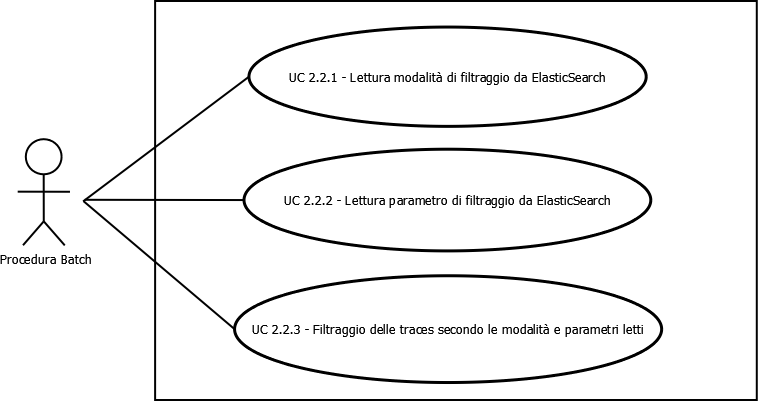
\includegraphics[width=13cm,height=13cm,keepaspectratio]{./img/UC2_2.png}
                    \caption{Esempio di caso d'uso}
                \end{figure}

                \begin{itemize}

                    \item \textbf{Attori} - Procedura \glossaryItem{Batch};
                    \item \textbf{Descrizione} - L'attore filtra le traces in base a parametri configurati e salvati in \glossaryItem{ElasticSearch};
                    \item \textbf{Precondizione} - I parametri per il filtraggio sono stati precedentemente configurati;
                    \item \textbf{Postcondizione} - Le traces sono state filtrate secondo i parametri configurati;
                    \item \textbf{Scenario principale}
                        \begin{enumerate}

                            \item L'attore legge la modalità di filtraggio da ElasticSearch (UC2.2.1);
                            \item L'attore legge il parametro di filtraggio da ElasticSearch (UC2.2.2);
                            \item L'attore filtra le traces secondo le modalità e i parametri letti (UC2.2.3).

                        \end{enumerate}

                \end{itemize}

\newpage

    \subsubsection{Progettazione} \label{progettazione}
		Questa attività, compito dei Progettisti, consiste nel design dell'architettura logica e dell'architettura in dettaglio del prodotto software da realizzare, perseguendo le seguenti caratteristiche qualitative:
			\begin{itemize}
				\item \textbf{sufficienza}: capacità di soddisfare tutti i requisiti documentati nell'\vAnalisiDeiRequisiti{};
				\item \textbf{comprensibilità}: capacità di essere capibile dai suoi utenti;
				\item \textbf{modularità}: suddivisione in parti chiare e distinte;
				\item \textbf{robustezza}: sopportazione di input dalla diversa natura, qualità e quantità;
				\item \textbf{semplicità}: avversione al superfluo;
				\item \textbf{incapsulazione}: identificazione di interfacce per la comunicazione che nascondano il funzionamento interno delle parti;
				\item \textbf{coesione}: raggruppamento delle parti rispetto a criteri che le avvicinino per scopo;
				\item \textbf{basso accoppiamento}: minimizzazione delle dipendenze ed assenza di dipendenze indesiderate.
			\end{itemize}

		L'attività di progettazione precede quella di codifica, permettendo di perseguire la correttezza per costruzione, con conseguenti vantaggi di efficienza ed efficacia.

		\myparagraph{Tecnica di progettazione} \label{tecnica_progettazione}

			La modellazione viene fatta utilizzando il linguaggio \glossaryItem{UML 2.0} in quanto standard nell'ambito dell'Ingegneria del Software. Questa scelta facilita la comunicazione con Committente, Programmatori, Responsabile e Verificatori.

			Viene fatto uso delle seguenti tipologie di diagrammi:
				\begin{itemize}
					\item \textbf{Diagrammi di package}: descrivono l'organizzazione dei package e degli elementi UML in essi contenuti, specificandone la visibilità; questi diagrammi permettono inoltre di esprimere dipendenze fra classi;
					\item \textbf{Diagrammi delle classi}: descrivono tipi di entità, mostrandone visibilità, attributi, operazioni e relazioni statiche;
					\item \textbf{Diagrammi di attività}: descrivono la logica procedurale delle attività, individuando come il flusso di controllo percorre certe azioni; questi diagrammi permettono inoltre di esprimere aspetti dinamici dei casi d'uso;
					\item \textbf{Diagrammi di sequenza}: descrivono una determinata sequenza di azioni, enfatizzando la collaborazione di un gruppo di oggetti al fine di implementare un certo comportamento.
				\end{itemize}

			Per la stesura dei diagrammi ci si avvale del programma Visual Paradigm 15.0 Community Edition poiché intuitivo da utilizzare ed impone il rispetto della grammatica UML 2.0.

		\newpage

		\myparagraph{Strategia di progettazione}

			La progettazione deve dominare la complessità del prodotto, portando ad una sua completa comprensione. Ciò è attuabile mediante una strategia \textit{divide et impera}, andando a scomporre il sistema in sottosistemi più semplici, che verranno a loro volta raffinati fino ad essere ridotti ad elementi atomici.

			Il requisito RVD4 su l'utilizzo di \glossaryItem{Spring Batch}, tuttavia, vincola la specifica architetturale ad adattarsi alle soluzioni offerte dal framework, specializzandole a proprio uso.	Per tanto, la progettazione avviene mediante un approccio \textit{Meet-in-the-middle}, che combina la decomposizione di problemi con la composizione di soluzioni. Un aspetto positivo è che ciò facilita l'individuazione e la specifica dei moduli perché basati su entità concrete fornite dai framework.

		\myparagraph{Stile di progettazione}

			Nel progettare si dovrà:
				\begin{itemize}
					\item perseguire l'\textit{Acyclic Dependency Principle}, eliminando le eventuali dipendenze circolari riscontrate nei digrammi di package mediante fattorizzazioni o riduzioni;
					\item sfruttare i \glossaryItem{design pattern}, risolvendo problemi già conosciuti con soluzioni progettuali già consolidate;
					\item tracciare ogni requisito funzionale al componente, quindi alla corrispettiva unità che lo realizza, così da garantire congruenza e completezza rispetto all'analisi dei requisiti effettuata;
					\item definire test di integrazione e di unità atti a verificare la conformità con quanto progettato;
					\item documentare mediante commenti UML, le scelte progettuali effettuate; in particolare vanno descritti: l'impiego di design pattern, i requisiti implementati, le dipendenze riscontrate e le interfacce definite;
					\item perseguire il principio dell'information hiding, al fine di raggiungere un'organizzazione propensa alla codifica in parallelo da parte di più Programmatori;
					\item nei diagrammi delle classi descrivere l'utilizzo di design pattern tramite commenti di colore rosso;
					\item segnalare le librerie e le API esterne; nei diagrammi delle classi farlo colorandole di arancione.
				\end{itemize}

\newpage

	\subsubsection{Codifica} \label{codifica}

		Questa attività, competenza dei Programmatori, consiste nella scrittura del codice sorgente di quanto progettato
		nell'attività di progettazione. Il codice deve compilare senza errori né warning. Deve inoltre rispettare le
		successive specifiche ed essere accompagnato da relativa documentazione per poter assicurare manutenibilità e leggibilità.

		\myparagraph{Nomenclatura}

			\begin{itemize}
				\item I nomi dei file devono essere tutti in minuscolo;
				\item i nomi di variabili e metodi devono avere la prima lettera minuscola;
				\item i nomi delle classi devono avere la prima lettera maiuscola;
				\item i nomi di costanti devono essere tutti in maiuscolo;
				\item i nomi di variabili, metodi e classi devono essere in \glossaryItem{camel case}.
			\end{itemize}
			
		\myparagraph{Commenti} \label{commenti}

			Classi e metodi devono essere preceduti da commenti secondo le convenzioni Javadoc:

			\begin{center}
				\url{http://www.oracle.com/technetwork/articles/java/index-137868.html}
			\end{center}

			Il codice va commentato per semplificarne la comprensione e la manutenzione; questo significa anche evitare
			di farlo quando ciò risulti ovvio.

			Inoltre:
			\begin{itemize}
				\item i commenti riguardo uno statement è preferibile che siano posizionati sopra lo statement stesso;
				\item una modifica del codice deve essere seguita da una modifica ai commenti che vi ci si riferiscono.
			\end{itemize}
		
		\myparagraph{Ricorsione}

			La ricorsione va evitata il più possibile. Ogni metodo ricorsivo dovrà essere accompagnato da una prova
			di terminazione e dall'analisi dell'occupazione della memoria. Risultati non soddisfacenti ne comporteranno il rifiuto.

\newpage

		\myparagraph{Formattazione} \label{formattazione}

			Il codice va formattato come da default in IntelliJ IDEA, consistente nello stile di
			indentazione K&R con indentazioni composte da 4 spazi, come mostrato dall'esempio qui sottostante:

			\lstset{language=Java}
			\begin{lstlisting}[frame=single]
public class Foo {
    public void foo(boolean a, int x, int y, int z) {
        do {
            try {
                if (x > 0) {
                    int someVariable = a ? x : y;
                    int anotherVariable = a ? x : y;
                } else if (x < 0) {
                    int someVariable = (y + z);
                    someVariable = x = x + y;
                } else {
                    for (int i = 0; i < 5; i++) doSmtng(i);
                }
                switch (a) {
                    case 0:
                        doCase0();
                        break;
                    default:
                        doDefault();
                }
            } catch (Exception e) {
                processException(e.getMessage(), x, z, a);
            } finally {
                processFinally();
            }
        }

        for (int i = 0; i < 5; i++) System.out.println(i);
    }

    private class InnerClass implements I1, I2 {
        public void bar() throws E1, E2 {
        }
    }
}
			\end{lstlisting}


\newpage

		\myparagraph{Codifica componente} \label{procedura_comp}

			Il seguente diagramma illustra la procedura da seguire per la codifica di un componente architetturale.
			
			\begin{figure}[!ht]
				\centering
				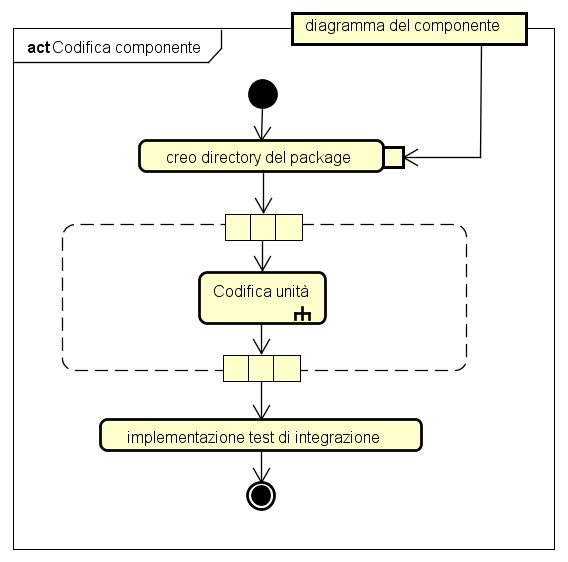
\includegraphics[scale=0.7]{./img/codifica_componente.png}
				\caption[Procedura di codifica di un componente]{Procedura di codifica di un componente}
			\end{figure}\\

\newpage

		\myparagraph{Codifica unità} \label{procedura_unit}

			Il seguente diagramma illustra la procedura da seguire per la codifica di un'unità architetturale.
			
			\begin{figure}[!ht]
				\centering
				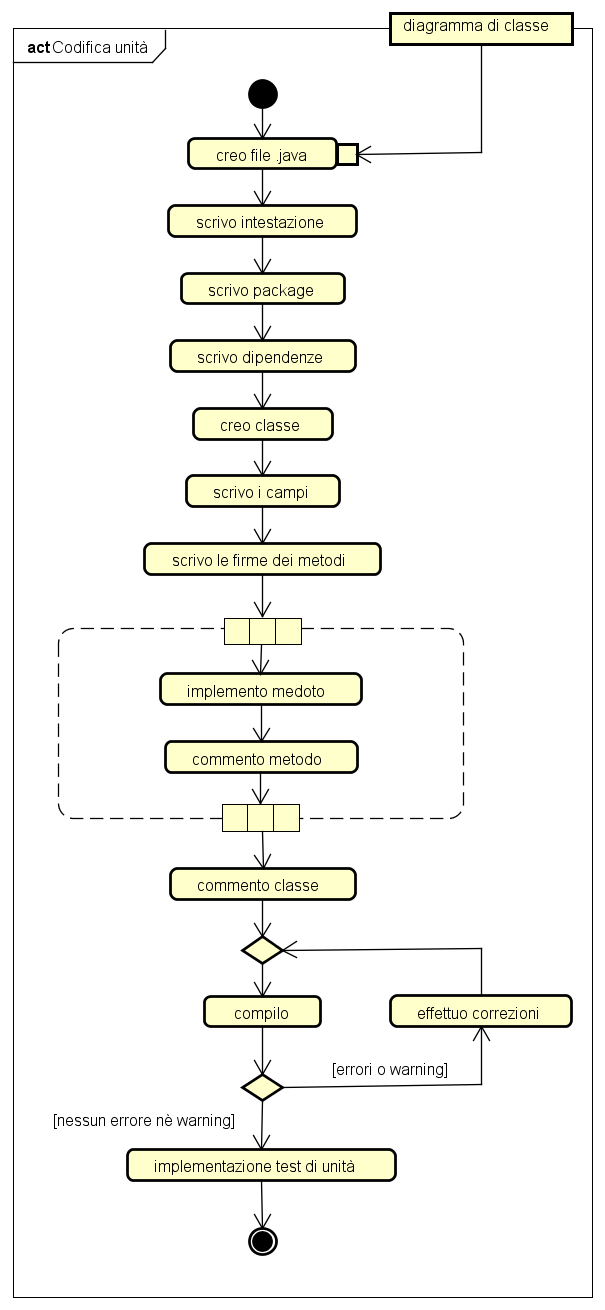
\includegraphics[scale=0.5]{./img/codifica_unita.png}
				\caption[Procedura di codifica di un'unità]{Procedura di codifica di un'unità}
			\end{figure}\\

\newpage

	\subsubsection{Strumentazione} \label{sviluppo_strumentazione}

		\myparagraph{SWEgo}

			\begin{figure}[htbp]
				\centering
				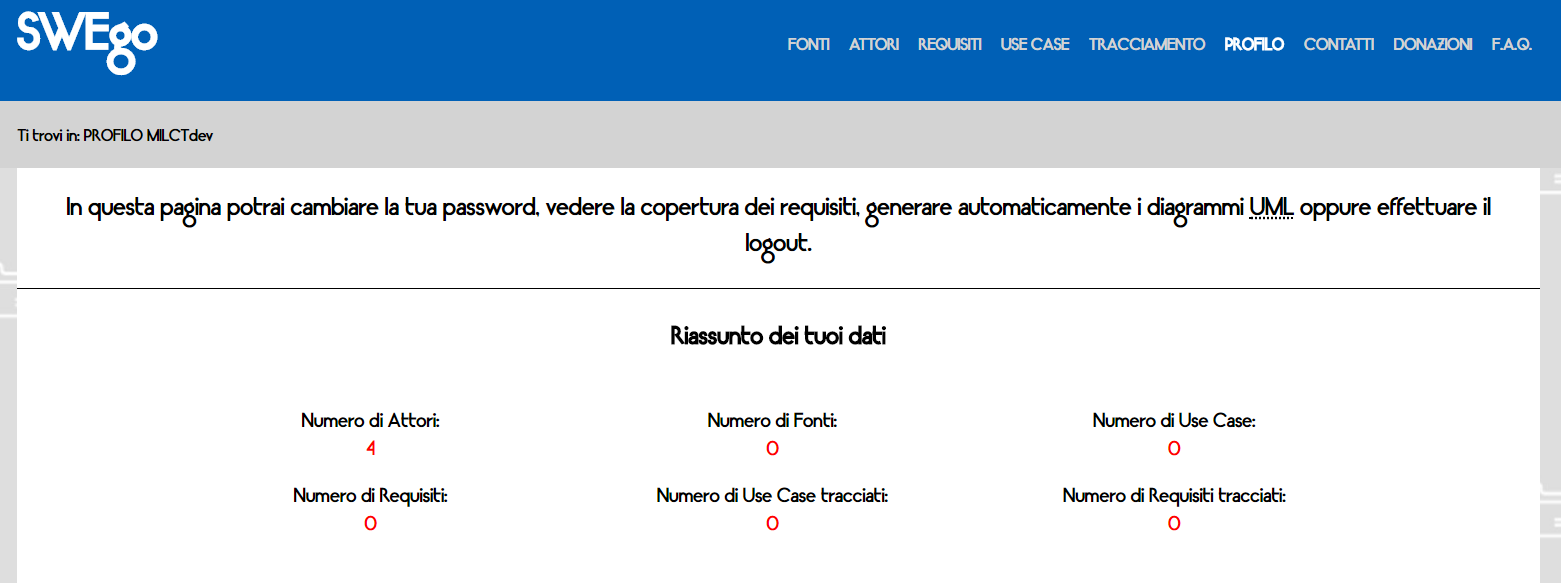
\includegraphics[scale=0.3]{./img/swego.png}
				\caption[SWEgo]{SWEgo: applicazione web utilizzata dal gruppo per il tracciamento dei requisiti}
			\end{figure}\\

			SWEgo è un potente strumento di tracciamento dei requisiti disponibile online. Esso offre una moltitudine
			di funzioni che semplificano e velocizzano il modo di produrre software.

\newpage

		\myparagraph{Papyrus}

			\begin{figure}[htbp]
				\centering
				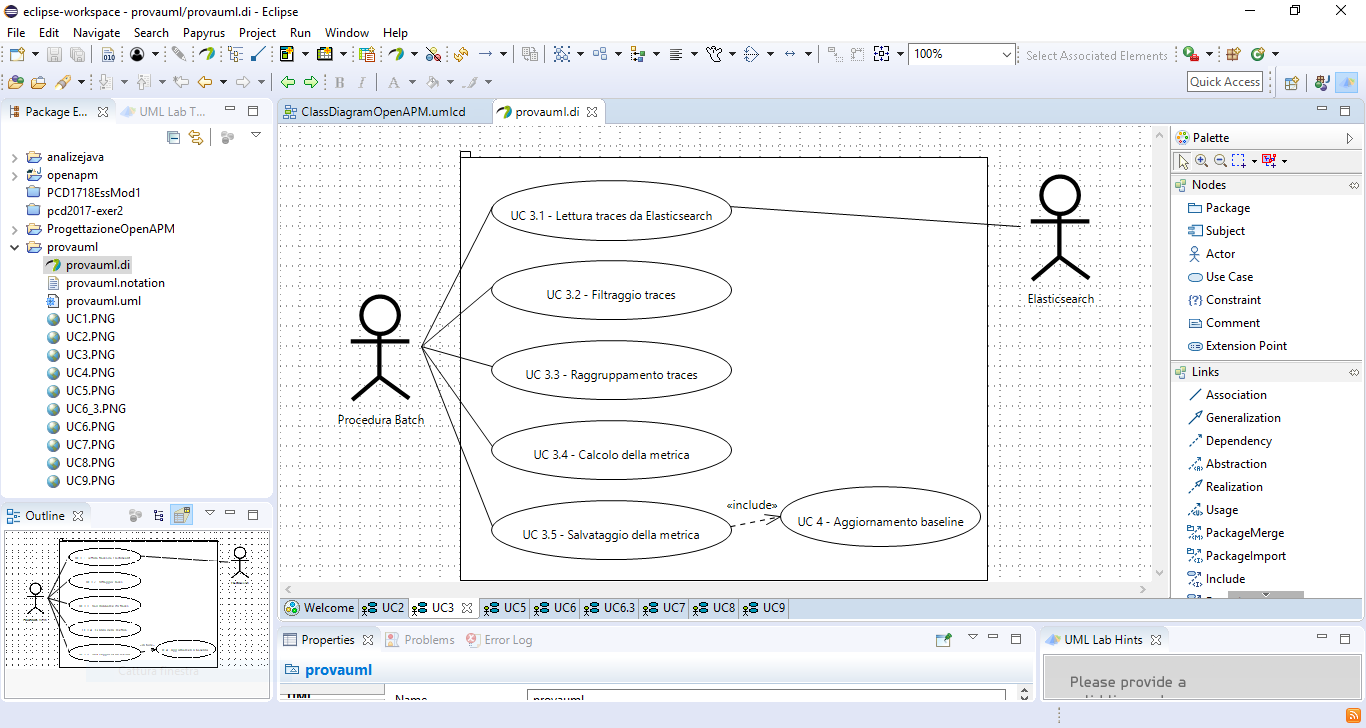
\includegraphics[scale=0.4]{./img/papyrus.png}
				\caption[Papyrus]{Papyrus: ambiente di modellazione UML utilizzata dal gruppo per disegnare i casi d'uso}
			\end{figure}\\

			Papyrus è un sofisticato e potente ambiente di modellazione UML integrato ad Eclipse; inizialmente utilizzato dal
			gruppo per disegnare casi d'uso, il suo utilizzo è stato accantonato perché risultava confusionario ai progettisti.

\newpage

		\myparagraph{Visual Paradigm 15.0 Community Edition}

			\begin{figure}[htbp]
				\centering
				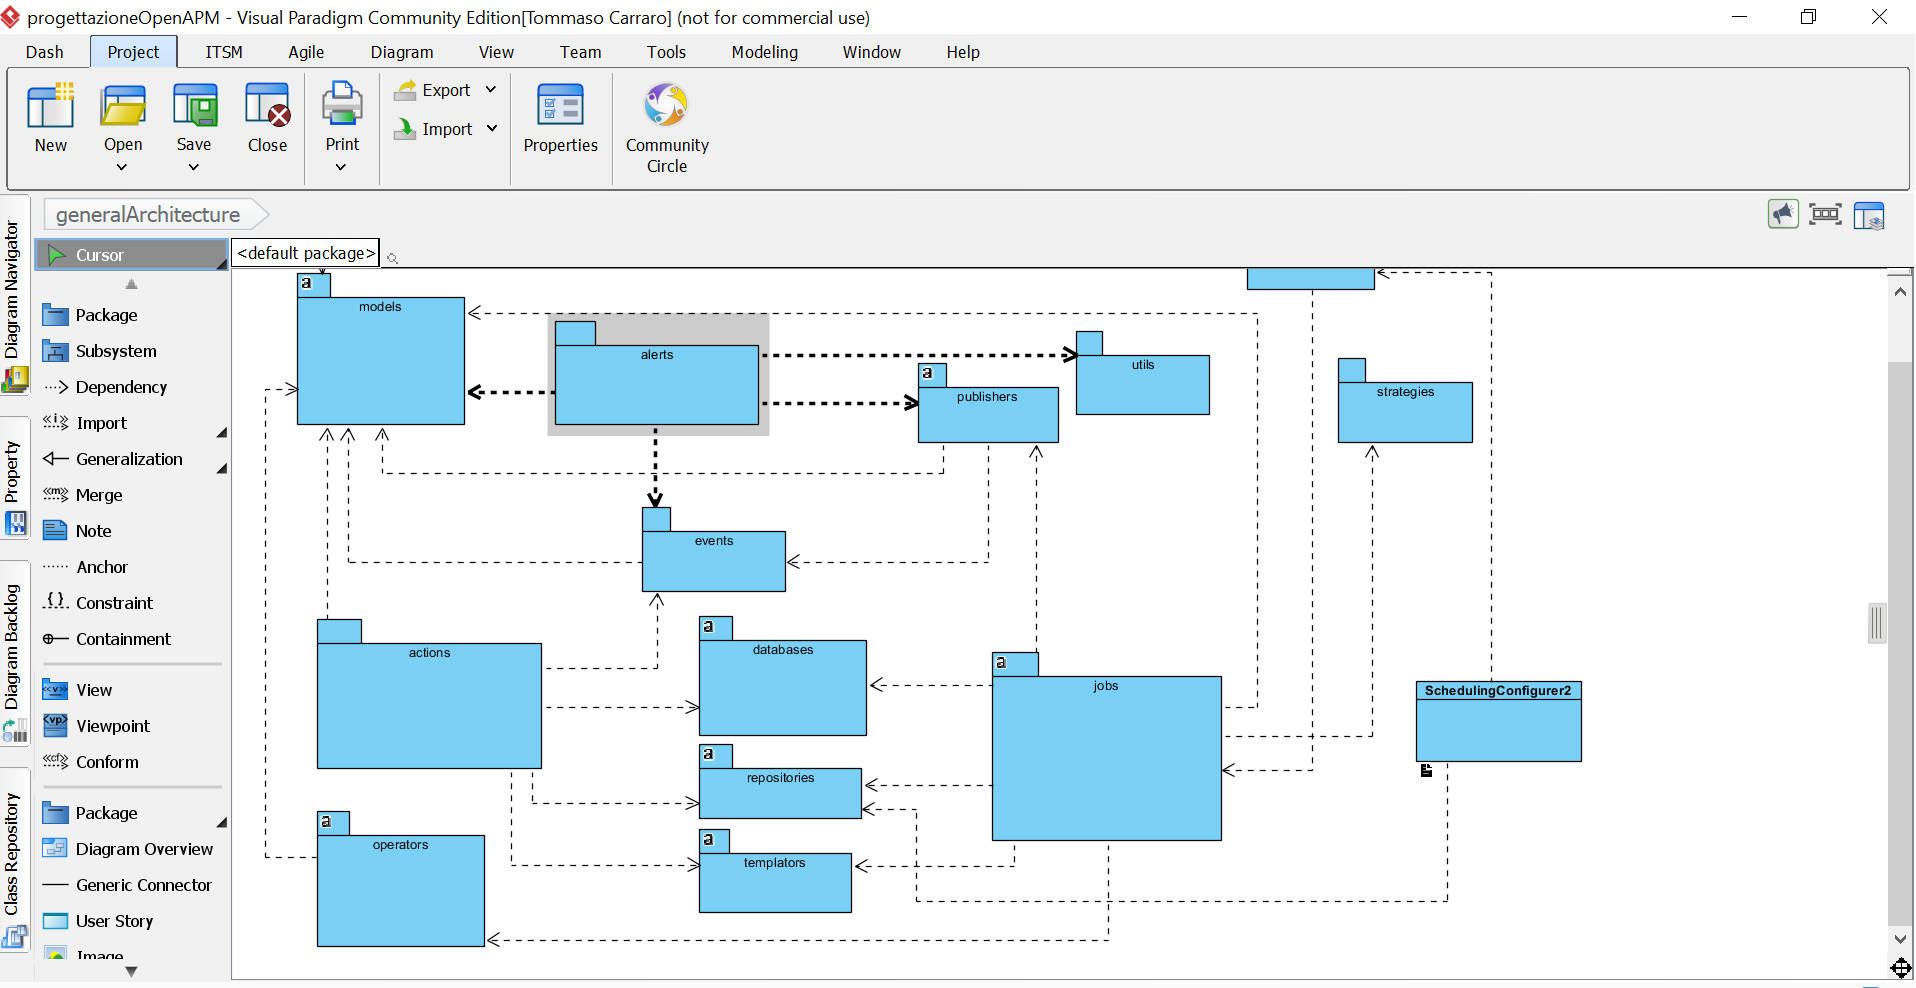
\includegraphics[scale=0.4]{./img/visualparadigm.png}
				\caption[Visual Paradigm 15.0 Community Edition]{Visual Paradigm 15.0 Community Edition:
				applicazione utilizzata dal gruppo per la modellazione UML}
			\end{figure}\\

			Visual Paradigm 15.0 Community Edition è stato scelto, a scapito di Papyrus a seguito di \textit{VI\_20180407.3},
			come applicazione per modellare diagrammi UML di classe e di sequenza per via della sua intuitività di utilizzo.

\newpage

		\myparagraph{IntelliJ IDEA}

			\begin{figure}[htbp]
				\centering
				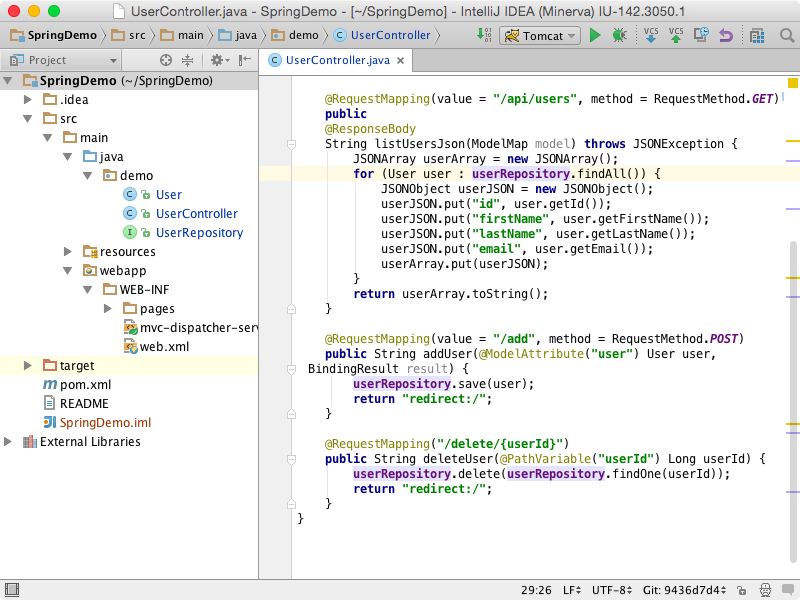
\includegraphics[scale=0.4]{./img/IntelliJ.png}
				\caption[IntelliJ IDEA]{IntelliJ IDEA: IDE utilizzato dal gruppo per la codifica del software}
			\end{figure}\\

			È un potente IDE che presenta integrazione con \glossaryItem{GitHub} e strumenti di analisi statica utili
			ai processi di supporto allo sviluppo. L'utilizzo dello stesso IDE, con la stessa configurazione, da parte di
			tutti i Programmatori preverrà o quantomeno faciliterà la soluzione di problemi riguardanti l'ambiente di sviluppo.
